% Chapter 1
% !TeX spellcheck = en_US 
\chapter{Introduction} % Main chapter title

\label{Chapter1} % For referencing the chapter elsewhere, use \ref{Chapter1} 
\setcounter{chapter}{1}
%----------------------------------------------------------------------------------------

% Define some commands to keep the formatting separated from the content 
\newcommand{\keyword}[1]{\textbf{#1}}
\newcommand{\tabhead}[1]{\textbf{#1}}
\newcommand{\code}[1]{\texttt{#1}}
\newcommand{\file}[1]{\texttt{\bfseries#1}}
\newcommand{\option}[1]{\texttt{\itshape#1}}
Underlying the success of artificial intelligence are learning algorithms, i.e.,
algorithms that learn from data to perform a certain task. We start by
two concrete examples of supervised learning algorithms. In the first example we
consider the problem of approximating functions from pointwise evaluations using linear regression. In the second example we look at the task of
classifying hand-written digits. In these two examples we identify and
familiarize ourselves with the main components of learning algorithms;
\emph{datasets}, \emph{a hypothesis class}, and \emph{optimization algorithms}.
We further identify important aspects of supervised learning algorithms, such as
overfitting, and underfitting. Finally, we motivate in these two examples
problems at the forefront of research in mathematical machine learning, namely
\emph{the curse of dimensionality (CoD)} and \emph{double/multiple descent phenomenon}. 
 
\section{Supervised Learning}
\subsection{Supervised Leaning Informally}
In supervised learning tasks the dataset $D$ is made up of
two components, input variables $D_x = \{x_i\}_{i = 1}^N$ and targets $D_y = \{y_i\}_{i=1}^N$. The dataset is assumed to be
generated by an unknown function $f: \text{input} \to \text{target}$. The goal in
a supervised learning task is to approximate the unknown function $f$ pointwise,
i.e., to find a function $h$ such that $h(x) \approx f(x)$ for any $x$, whether
it belongs to $D_x$ or not. The target value can take finitely many values,
e.g., $\text{target} \in \{0,1, \dots, M\}$. In such a case, the supervised
learning task is called a \emph{classification task}. If the target can take
infinitely many values, the learning task is called a \emph{regression task}.  
Supervised learning problems are approached by first choosing a \emph{hypothesis
space} $\mathfrak{H}$, in which one looks for an approximation to the unknown function $f$. For example, if the data $x$ is one-dimensional and the target
take values in $\mathbb{R}$ one can define the hypothesis class to be the set of
all affine mappings, i.e., 
\begin{equation}
    \label{eq:affine_mappings}
\mathfrak{H} = \bigl\{f \ | \ f(x) = ax + b, \ a, b, \in \mathbb{R}    
\bigr\}.
\end{equation}

Then, one define a loss function $l$ that measures how well a hypothesis
function $h$ approximates an unknown function $f$ at a point $x$. Using the
dataset $D$, the supervised learning
problem can be then formulated as an optimization problem 
\begin{equation}
    \min_{h \in \frak{H}} \frac{1}{N}\sum_{i=1}^{N}l(h(x_i), y_i).
\end{equation}

While there are many alternatives to solve these optimization problems, the
by-far most used algorithms are variants of the gradient-descent algorithm. 

Let's look at some concrete examples. 

\begin{boxedexample}[Regression] \complementary{\theexample}
    \label{ex:regression}
    Let $x$ be a random variable that takes values in the interval $[-1,1]$. And assume we
    have access to a dataset $D = \{(x_i, y_i)_{i=1}^{200}\}$ generated by the unknown
    function 
    $$
    f(x) = x^2 \cos(5x) \exp(-x).
    $$ 
    Assume that the dataset is corrupted by Gaussian noise.
    To learn a function $h$ that approximates $f$ let your hypothesis class be
    the class of affine functions \eqref{eq:affine_mappings}. Let the loss
    function be the absolute error, i.e., 
    \begin{align*}
    l(h(x_i), y_i) &= |h(x_i)- y_i| \\
& = |ax_i + b - y_i|.
    \end{align*}
    Use a gradient-descent-like algorithm to choose the best hypothesis $h$,
    i.e., the best scalars $a$ and $b$. 

    Change your hypothesis class to the class of all polynomials up to   order
    20 and repeat the optimization process. Which class is better for
    optimization? \autoref{fig:regression} shows the outcome of such an experiment.
\end{boxedexample}
\begin{figure}[htbp]
    \centering
    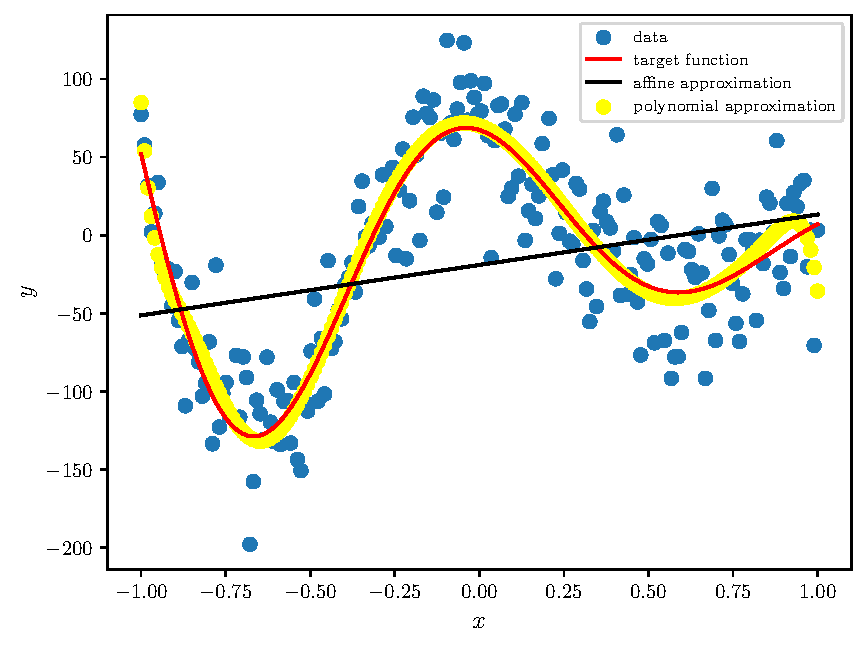
\includegraphics[width=0.8\textwidth]{Regression.pdf}
    \caption{A regression task; the goal is to fit noisy data (blue dots) assumed to be generated from a true function (solid red line). The data is fitted using an affine mapping (solid black line) and a polynomial mapping (solid yellow line).}
    \label{fig:regression}
\end{figure}   

\begin{boxedexample}[Classification] \complementary{\theexample}
    \label{ex:classification}
\end{boxedexample}

\autoref{fig:regression} shows two hypotheses, one linear and one nonlinear, that we learned to fit the data in
\autoref{ex:regression}. The figure depicts an interesting phenomenon; a certain
hypothesis $h$ can fit the data too accurately; notice for example in
\autoref{fig:Regression} that the polynomial-regression model fits badly local
minima of the target function. In these regions, it is optimized to fit the
noise. The outcome of such a result is that the polynomial-regression model will
fail to generalize well in these regions, i.e., it will have large error on
unseen data in these regions. This is called \emph{overfitting}.
On the other hand, the linear-regression model produces largely deviated from
the data everywhere, and would, hence, also generalizes badly to unseen data.
This is called an \emph{underfitting} phenomenon. 

Think about the influence of the following factor on the underfitting and
overfitting:
\begin{itemize}
    \item Complexity of the model. For a polynomial-regression model this can be
    the degree of the polynomial. 
    \item Size of the dataset. For example, would adding more data decrease or
    increase underfitting?
\end{itemize}

\subsection{Supervised Learning Formally}
A formal definition of learning.

\section{Curse of Dimensionality}
Programming exercise and theorem about approximating smooth functions in higher
dimensions. 
\begin{boxedexample}[Classification] \complementary{\theexample}
    \label{ex:CoD}
tba.
\end{boxedexample}

\section{Approximating Highly-Oscillatory Functions}
\begin{boxedexample}[Classification] \complementary{\theexample}
    \label{ex:oscillatory}
    tba.
\end{boxedexample}

\section{Validity of Ocaam Razor and Double-Descent Phenomenon}
\begin{boxedexample}[Double descent] \complementary{\theexample}
    \label{ex:double_descent}
    tba.
\end{boxedexample}

\section*{Wait! What is what?}
Here is a list of questions that help you check your understanding of key
concepts inside this chapter?

%----------------------------------------------------------------------------------------
